\documentclass[sigconf,authoryear]{acmart}

% Packages
\usepackage{graphicx}
\usepackage{amsmath}
\usepackage{hyperref}
\usepackage{totpages}
\usepackage{natbib}
\usepackage{float}
\usepackage{afterpage}

% Metadata Information
\title{Mechanistic Interpretability of Large Language Models: A Survey}

\author{Pradyumna Shyama Prasad}
 
% Remove conference-related metadata
\settopmatter{printacmref=false} % Removes citation information below abstract
\renewcommand\footnotetextcopyrightpermission[1]{} % Removes footnote with conference info
\pagestyle{plain} % Removes running headers

% This suppresses the conference info completely
\acmConference[]{}{}{} % Suppresses conference info
\acmYear{} % Removes the year
\acmISBN{} % Removes ISBN
\acmDOI{} % Removes DOI

\setcitestyle{authoryear,round}

\begin{document}

\begin{abstract}
  This survey provides a comprehensive overview of mechanistic interpretability in large language models (LLMs), focusing on techniques to understand the internal computations and decision-making processes of neural networks, transformers, and other complex architectures. We introduce key concepts such as features, polysemanticity, and circuits, which form the foundation for understanding model behavior at a granular level. The paper explores a taxonomy of approaches, categorizing them into observational techniques like probing and sparse autoencoders, and interventional techniques such as ablation and activation patching. We review recent advances in these areas, discussing how they contribute to uncovering the underlying mechanisms of LLMs.

  We address the challenges of scaling interpretability techniques to larger and more complex models, highlighting issues such as computational feasibility and the difficulty of disentangling polysemantic features. We examine the current limitations of interpretability methods and their implications for AI transparency and safety. Furthermore, we identify open questions and potential future directions for research, including the development of more robust evaluation metrics and approaches for generalizing interpretability across different tasks and model architectures.
  
  
  
  \end{abstract}



% Keywords
\keywords{Mechanistic interpretability, deep learning, neural networks, transformers, interpretability, AI, challenges, future directions}

\maketitle

\section{Introduction}

\subsection{Background and Motivation}
Since the advent of the Transformer \citep{vaswani2023attentionneed}, language models have achieved near-human abilities on various tasks, from mathematics to programming \citep{qwen2math2024,dubey2024llama3herdmodels,openai2024gpt4technicalreport}. However, their interpretability has not kept pace with their capabilities, posing challenges for safety, transparency, and trust in high-stakes applications.

While existing interpretability methods focus on input-output relationships and high-level summaries \citep{zhao2023explainabilitylargelanguagemodels, bolukbasi2021interpretabilityillusionbert}, mechanistic interpretability aims to reverse-engineer neural networks, making their internal behavior understandable \citep{olah2020zoom}. This approach is crucial for debugging models, identifying biases, and ensuring reliable and ethical AI systems \citep{räuker2023transparentaisurveyinterpreting}.

The need for mechanistic interpretability has become increasingly urgent as language models grow in size and capability. As \citet{bereska_mechanistic_2024} argue, understanding the internal mechanisms of these models is essential for ensuring their alignment with human values and avoiding potential catastrophic outcomes. Mechanistic interpretability offers several key benefits. Firstly, it enhances safety and alignment by providing insights into model decision-making processes, which can help identify and mitigate potential safety risks, such as deceptive or misaligned behaviors \citep{bereska_mechanistic_2024}. Secondly, it improves robustness and generalization; understanding internal model mechanisms can lead to improvements in these areas, as highlighted by \citet{rai2024practicalreviewmechanisticinterpretability}. Lastly, it enables targeted improvements, as mechanistic insights allow for more precise and effective model modifications, enabling researchers to enhance specific capabilities or correct undesired behaviors \citep{rai2024practicalreviewmechanisticinterpretability}.

However, mechanistic interpretability faces significant challenges with modern deep learning architectures. Large language models like GPT-3, with 175 billion parameters, are difficult to interpret due to their size and complexity, with individual neurons often representing multiple, overlapping features. Moreover, the field remains pre-paradigmatic, lacking widely accepted definitions for many key concepts \citep{bereska_mechanistic_2024}.

Despite these challenges, the potential benefits of mechanistic interpretability make it a crucial area of research as we continue to develop and deploy increasingly powerful AI systems. This survey aims to provide a comprehensive overview of current mechanistic interpretability techniques, their applications, and the challenges they face in the context of large language models.

\subsection{Scope of the Survey}

This survey focuses on mechanistic interpretability in large language models (LLMs), aiming to uncover and explain their internal structures and computations. Unlike general interpretability methods that emphasize input-output mappings, we explore techniques that investigate the internal workings of these models. Key aspects covered in this survey include feature representation across LLM layers, circuits and modular computation within models, and the challenges posed by polysemanticity and superposition. We also discuss interventional techniques for causal analysis, as well as the scalability of interpretability methods to models with billions of parameters.


\subsection{Contributions of This Survey}

Recent surveys have significantly advanced the field of mechanistic interpretability (MI). Notably, \citet{rai2024practicalreviewmechanisticinterpretability} provided a practical review focusing on techniques and applications in transformer-based models, while \citet{bereska_mechanistic_2024} offered an AI safety-focused analysis of MI across various AI systems. Our work complements these surveys and offers distinct contributions: 

\begin{enumerate}
    \item \textbf{Comparative Overview:}
    \begin{itemize}
        \item \citet{rai2024practicalreviewmechanisticinterpretability}: A practical guide for beginners, with detailed coverage of MI techniques and their implementations in transformer models.
        \item \citet{bereska_mechanistic_2024}: A broader analysis of MI, emphasizing AI safety across different systems beyond language models.
        \item Our survey: Bridges these approaches by focusing specifically on large language models (LLMs), offering both practical and theoretical insights.
    \end{itemize}

    \item \textbf{In-depth Analysis of Sparse Autoencoders (SAEs):} Previous surveys mention SAEs, but our work provides a detailed examination of SAEs in the context of LLM interpretability. We explore their theoretical foundations, practical implementations, and potential to disentangle polysemantic features in LLMs, offering a more comprehensive analysis of this emerging technique.

    \item \textbf{Focus on Intervention Techniques:} Our survey reviews interventional methods, including activation patching, causal tracing, and causal scrubbing, synthesizing recent developments and highlighting their strengths, limitations, and applications for understanding LLM internals. This complements the broader technique coverage in \citet{rai2024practicalreviewmechanisticinterpretability} and the safety implications discussed in \citet{bereska_mechanistic_2024}.

\end{enumerate}

By providing specific insights and synthesizing practical and theoretical perspectives, our survey offers a focused yet comprehensive view of key frontiers in mechanistic interpretability for large language models. This complements existing literature by providing a specialized perspective on emerging techniques and their applications in understanding LLM internals.


\section{Key Concepts and Definitions}
\subsection{Features are the Fundamental Units of Representation}
Features are the fundamental units of representation in neural networks, encapsulating specific patterns or properties of input data. They are encoded within neuron activations across different layers, forming the building blocks of how a model processes and understands data. In transformer-based models, features are represented in layers of attention heads, feed-forward networks, and residual streams.

A \textbf{feature} can be thought of as a specific input property, such as recognizing a linguistic pattern or detecting an edge in an image. For example, researchers found a neuron that activates only for French text, demonstrating a clear correspondence between the neuron and a specific feature \citep{gurnee2023findingneuronshaystackcase}.

\subsubsection{Polysemanticity}

It is not always the case that one neuron will correspond to a single feature. Many neurons in deep learning models exhibit \textbf{polysemanticity}, meaning they activate in response to multiple unrelated features. For instance, a neuron may fire when processing both ``French text'' and ``Base64-encoded text,'' or respond to different concepts in distinct contexts. For example, out of over 300,000 neurons in GPT-2, researchers at OpenAI were able to find explanations that explained over 50\% of the variance for only about five thousand neurons (only 1.6\% of them) \citep{LawrenceC2024,bills2023language}.   


One hypothesis for why this occurs because neural networks often need to represent more features than there are available neurons \citep{elhage2022superposition}. As a result, some neurons encode multiple features simultaneously, leading to complex activation patterns that do not correspond to just one interpretable concept. Understanding polysemanticity is a major challenge for neural networks because they exponentially increase the number of combinations of neurons needed to understand a feature. For example, if there is one neuron with five different possible features, which connects to another neuron with five other different features, that is 25 different combinations that need to be considered. \citep{olah2020zoom}  



\subsubsection{Superposition}
One hypothesized cause for polysemanticity is \textbf{superposition}. As explained above, superposition is when a neural network represents more features than it has dimensions. Superposition occurs when a neural network represents more features than the number of available neurons (or dimensions) in its layers. In other words, the network must "compress" multiple features into the same set of neurons. This leads to a situation where individual neurons activate for multiple, potentially unrelated features, contributing to polysemanticity.

Superposition can be thought of as a method for the neural network to efficiently store and process a large number of features with a limited number of neurons. Instead of dedicating a neuron to a single feature, the network encodes several features into overlapping directions in the activation space. While this allows the model to represent more information with fewer resources, it also makes it harder to interpret because each neuron is no longer aligned with a distinct, interpretable feature.

\subsection{Circuits}
A circuit is a subgraph within a neural network connecting neurons or features across layers, forming a coherent, interpretable mechanism. Circuits reveal how individual neurons contribute to higher-level functions, providing insights into specific computations and feature detection patterns.

\subsubsection{Circuits in Transformers}
In transformers, circuits are pathways through which attention heads, tokens, and layers interact to compute functions like attention patterns and predictions. The \textit{residual stream} enables information flow, creating a modular and compositional structure.

\subsubsection{Attention Heads and Circuits}
Attention heads act as sub-circuits, facilitating information transfer between tokens through the \textbf{query-key-value (QKV)} mechanism:
\begin{itemize}
    \item \textbf{QK Circuits} govern which tokens attend to each other.
    \item \textbf{OV Circuits} determine a token's influence on final predictions.
\end{itemize}

\begin{figure}
  \centering
  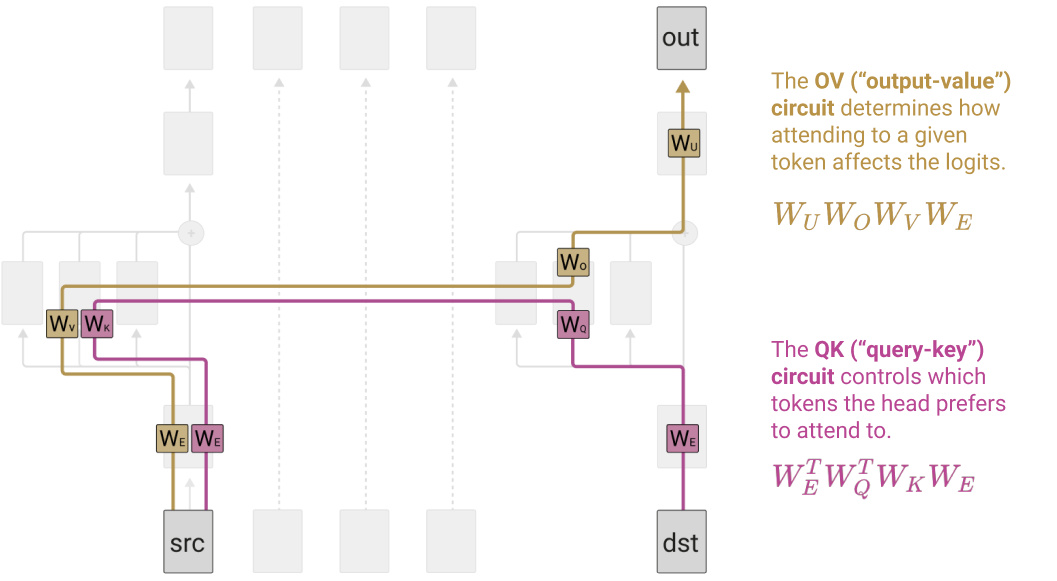
\includegraphics[width=0.9\columnwidth]{transformer_circuit_example.png}
  \caption{An example of a circuit in a transformer model. From \citep{olah2020zoom}} 
  \label{fig:figurelabel}
\end{figure}

\subsubsection{Residual Stream and Information Flow}
The residual stream acts as the communication backbone for circuits in transformers, enabling interaction between attention heads and layers. This allows for \textbf{higher-order circuits}, forming sophisticated representations and complex dependencies between tokens.

\begin{figure}
  \centering
  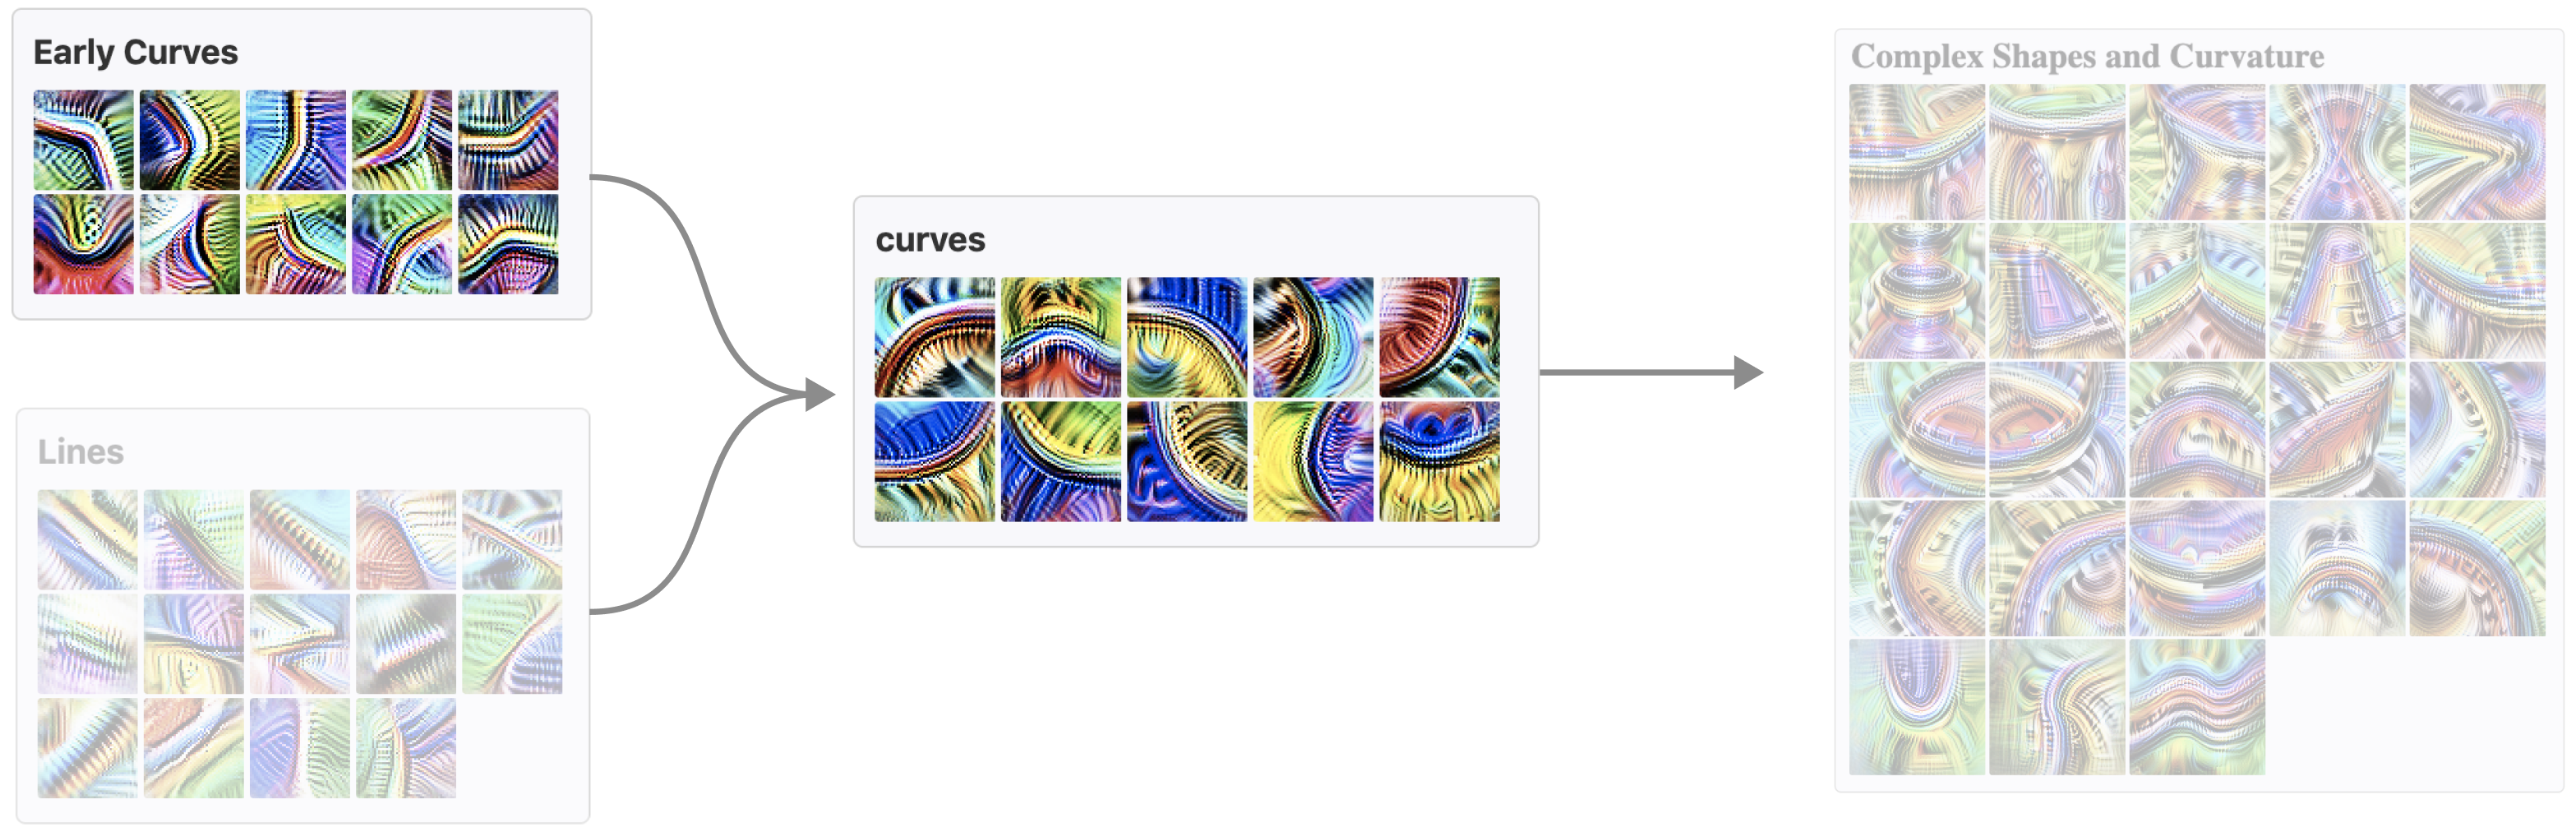
\includegraphics[width=0.9\columnwidth]{circuit_example.png}
  \caption{An example of a circuit in a CNN model. From \citep{olah2020zoom}} 
  \label{fig:figurelabel}
\end{figure}


\section{Taxonomy of Approaches}
We draw on two previously existing reviews to classify approaches in mechanistic interpretability \citep{bereska_mechanistic_2024, rai2024practicalreviewmechanisticinterpretability}. Based on these existing frameworks, we classify techniques in mechanistic interpretability into two types: \textbf{observational techniques} and \textbf{interventional techniques}. 
\subsection{Observational Techniques} 
\subsubsection{Probing} 

Probing is a diagnostic technique used to reverse engineer the internal representations of neural networks, particularly in NLP. It involves training simple classifiers (probes) to predict specific properties from the activations of hidden layers or individual neurons. These properties can range from linguistic features to abstract information like spatial and temporal relationships.

Probing offers insight into the latent knowledge encoded by neural models, revealing how well internal representations capture targeted properties and how these properties are distributed across neurons and layers \citep{zhao2023explainabilitylargelanguagemodels, bolukbasi2021interpretabilityillusionbert}. This helps in understanding how neural networks encode and process information at various levels of abstraction.

\subsubsection{Variations within Probing}

\paragraph{Linear Probing:} The most common form, using simple linear classifiers to predict properties. \citet{gurnee2024languagemodelsrepresentspace} used linear ridge regression to predict spatial-temporal information, while \citet{marks2024geometrytruthemergentlinear} classified true and false statements, finding distinct linear directions in the model's representation space.

\paragraph{Nonlinear Probing:} Uses more complex classifiers like MLPs to capture nonlinear relationships. \citet{gurnee2024languagemodelsrepresentspace} found minimal improvements over linear probes for spatial-temporal features, highlighting concerns about overfitting and reduced interpretability.

\paragraph{Sparse Probing:} Introduces sparsity constraints to identify specific neurons encoding target features. \citet{gurnee2023findingneuronshaystackcase} demonstrated its effectiveness in analyzing large language models, uncovering key neurons for detecting specific features like language type or code structure.

Sparse probing helps address the challenge of \textbf{polysemanticity}, where neurons activate for multiple, often unrelated features. By focusing on a smaller set of neurons, it reduces interference from polysemantic neurons and offers a clearer view of feature representation \citep{olah2020zoom}.

\subsubsection{Limitations of Probing}

Recent studies have identified several limitations:

\begin{itemize}
    \item Probe quality doesn't necessarily indicate neuron importance. \citet{antverg2022pitfallsanalyzingindividualneurons} argue that a well-performing probe may still rank neurons inaccurately.
    \item Distinction between encoded and actively used information. Identifying neurons that encode information doesn't guarantee their use in model predictions \citep{antverg2022pitfallsanalyzingindividualneurons}.
    \item Lack of causal interventions to determine essential neurons for model decisions \citep{elhage2022superposition}.
\end{itemize}

These limitations highlight the need for caution when interpreting probing results and the importance of complementary techniques in mechanistic interpretability \citep{bereska_mechanistic_2024, rai2024practicalreviewmechanisticinterpretability}.
\begin{table}[h]
  \centering
  \footnotesize
  \begin{tabular}{|p{2.5cm}|c|c|c|c|}
  \hline
  \textbf{Study} & \textbf{Linear} & \textbf{Nonlinear} & \textbf{Sparse} & \textbf{Other} \\
  \hline
  Gurnee et al. (2024) & \checkmark & \checkmark & & \\
  \hline
  Marks et al. (2024) & \checkmark & & & \\
  \hline
  Gurnee et al. (2023) & & & \checkmark & \\
  \hline
  Antverg et al. (2022) & & & & \checkmark \\
  \hline
  \end{tabular}
  \caption{Types of Probing Techniques Used in Recent Studies}
  \label{tab:probing_techniques_used}
  \end{table}

  \subsubsection{Sparse Autoencoders}

  Sparse autoencoders (SAEs) have emerged as a powerful tool for addressing the challenges of interpreting large language models, particularly the issue of polysemanticity. While traditional probing methods struggle with causal clarity and the complexity of these models, SAEs offer a novel approach by encouraging sparsity in neural representations.
  
  SAEs are a type of autoencoder that enforces sparsity in its latent space representation. Unlike traditional autoencoders, which compress input data into a dense latent representation, SAEs ensure that only a small number of neurons in the hidden layer are activated for any given input. This is typically achieved by adding a regularization term to the loss function that penalizes dense activations. The goal is to force the network to learn more efficient, distinct features by reducing redundancy and ensuring that each neuron in the hidden layer captures a unique aspect of the data \citep{cunningham2023sparseautoencodershighlyinterpretable, bricken2023monosemanticity}.
  
  The key advantage of SAEs in interpreting large language models is their ability to mitigate polysemanticity. By activating only a subset of neurons for each input, SAEs encourage each neuron to represent a distinct and interpretable feature, rather than encoding multiple overlapping or unrelated features. This makes it easier to trace connections between neurons and specific concepts, leading to more interpretable and monosemantic representations.
  
  \paragraph{Advantages of SAEs} Recent work by \citet{bricken2023monosemanticity} demonstrated the power of SAEs in learning disentangled features from transformer models. Using a large dataset of 8 billion data points, they decomposed MLP layer activations into sparse, monosemantic features responding to specific contexts such as Arabic script, DNA sequences, base64 strings, and Hebrew script. These features exhibited \textbf{high specificity} and \textbf{sensitivity} for the contexts they represented, demonstrating the ability of SAEs to produce clearer and more interpretable features than individual neurons.
  
  \paragraph{Recent Advancements} The use of SAEs is particularly effective when compared to traditional probing methods. While probing often lacks causal clarity and may conflate correlation with causation, SAEs enforce a latent space where each feature is monosemantic. This means that each activation has a clear and interpretable relationship with a specific concept, making it easier to reverse-engineer the decision-making processes of large models by attributing behaviors to distinct learned features \citep{cunningham2023sparseautoencodershighlyinterpretable, bricken2023monosemanticity}.
  
  \paragraph{Validation Methods} To validate the reliability and specificity of these features, \citet{bricken2023monosemanticity} and \citet{cunningham2023sparseautoencodershighlyinterpretable} designed computational proxies that estimate the likelihood of certain contexts being present in the data. By correlating the activations of SAEs with these proxies across a large dataset of over 8 billion tokens, they demonstrated that the features learned by the SAE were indeed highly specific to the target contexts. The sparse autoencoder model consistently activated the correct feature when the context was present, reducing the risk of polysemantic neurons confusing different features.
  
  \paragraph{Scaling to Larger Models} Recent efforts have scaled the SAE framework to larger models, addressing the critical challenge of interpretability in state-of-the-art language models. \citet{lieberum2024gemmascopeopensparse} applied SAEs to Gemma 2 models (ranging from 2B to 27B parameters), enabling a layer-wise application of SAEs across different model architectures. The authors also introduced the \textit{JumpReLU} activation function, which dynamically adjusts the number of active neurons based on the input, further refining the specificity and interpretability of the learned features. This framework allows researchers to conduct detailed circuit analysis and understand how model representations evolve across layers, providing a broader picture of how sparse autoencoders perform in large-scale models.
  
  \paragraph{Limitations and Challenges} However, SAEs are not without limitations and challenges. \citet{chaudhary2024evaluatingopensourcesparseautoencoders} found that while SAEs could disentangle features in smaller models like GPT-2 Small, their performance often degraded the model's factual knowledge when applied to certain tasks, such as separating a city's country and continent. This highlighted the limitations of SAEs in some tasks, especially in comparison to supervised methods like Distributed Alignment Search (DAS), which performed better at disentangling factual knowledge.
  
  \paragraph{Promise and Potential} Additionally, \citet{makelov2024principledevaluationssparseautoencoders} addressed these concerns by evaluating SAEs on principled grounds, noting that while SAEs can provide monosemanticity, their performance is highly sensitive to model architecture and the specific task. In their experiments with the IOI (Indirect Object Identification) task, the SAE models demonstrated reasonable disentanglement of features but still faced challenges with preserving the model's overall performance, revealing that more work is needed to balance feature sparsity with model fidelity.
  
  \paragraph{Universality of SAEs} Despite these challenges, SAEs have shown promise in learning higher-level representations that span multiple neurons, capturing complex, real-world features more effectively than individual neurons. This is significant because individual neurons, particularly in deep models, frequently fail to capture complex, real-world features due to polysemanticity. By spanning multiple neurons, SAEs learn more meaningful and contextually accurate representations, such as identifying languages or specific encoding formats, making the internal mechanics of the model more transparent \citep{cunningham2023sparseautoencodershighlyinterpretable, bricken2023monosemanticity}.
  
  \paragraph{Future Directions} Furthermore, SAEs exhibit \textbf{universality}, meaning that the learned features remain consistent across multiple runs and different models. This was demonstrated in \citet{bricken2023monosemanticity}, where the same features could be extracted by the SAE across different models, further reinforcing the interpretability and reliability of the learned representations. The public release of these models and their learned features \citep{lieberum2024gemmascopeopensparse} has made it easier for other researchers to explore and apply SAEs to a wide range of interpretability tasks.
  
  Future research directions for SAEs in mechanistic interpretability include several key areas. \textbf{Developing techniques to maintain model performance while increasing feature interpretability} is an important goal, ensuring that interpretability improvements do not come at the cost of model efficacy. \textbf{Exploring the application of SAEs to other model architectures beyond transformers} could uncover new insights across different AI systems. Researchers should also focus on \textbf{investigating ways to combine SAEs with other interpretability methods} for a more comprehensive understanding of model behavior. \textbf{Creating standardized benchmarks for evaluating the quality and utility of SAE-learned features} will help in assessing their effectiveness. Finally, \textbf{studying the potential of SAEs in improving model robustness and out-of-distribution generalization} can lead to more reliable AI systems.
  
\begin{table}[h]
  \centering
  \footnotesize
  \begin{tabular}{|p{2cm}|p{2.5cm}|p{2.5cm}|}
  \hline
  \textbf{Study} & \textbf{Key Contribution} & \textbf{Findings/Implications} \\
  \hline
  Bricken et al. (2023) & Applied SAE to transformer MLP layers & 
  Decomposed activations into monosemantic features (e.g., Arabic script, DNA sequences) \\
  \hline
  Cunningham et al. (2023) & Validated SAE features with computational proxies & 
  Demonstrated high specificity of learned features \\
  \hline
  Lieberum et al. (2024) & Scaled SAE to larger models (Gemma 2) & 
  Introduced JumpReLU activation for dynamic neuron activation \\
  \hline
  Chaudhary et al. (2024) & Evaluated open-source SAEs & 
  Found limitations in certain tasks (e.g., separating city's country and continent) \\
  \hline
  Makelov et al. (2024) & Principled evaluation of SAEs & 
  Noted sensitivity to model architecture and specific tasks \\
  \hline
  \end{tabular}
  \caption{Summary of Sparse Autoencoder (SAE) Studies and Their Contributions}
  \label{tab:sae_studies}
  \end{table}

  \subsection{Interventional Techniques}

  While observational techniques provide insights into neuron activations, they may only reveal correlations rather than causal relationships. Interventional techniques address this by altering neuron activations to observe changes in model output \citep{bereska_mechanistic_2024,rai2024practicalreviewmechanisticinterpretability}.
  
  \subsubsection{Ablation techniques}
  
  Ablation techniques explore causal relationships by systematically removing or deactivating model components and observing the effect on task performance. This helps identify components of computational circuits performing specific tasks, providing causal evidence for their existence \citep{wang2022interpretabilitywildcircuitindirect, hanna2023doesgpt2computegreaterthan}.
  
  For example, ablating attention heads in transformers can determine their necessity for tasks like indirect object identification (IOI). A significant performance drop when ablating a Name Mover Head suggests its role in a circuit for copying correct tokens \citep{wang2022interpretabilitywildcircuitindirect}. Similarly, ablations in GPT-2 identified specific neurons and layers critical for mathematical operations like greater-than comparisons \citep{hanna2023doesgpt2computegreaterthan}.
  
  However, complete component removal may introduce unintended effects, motivating more refined methods like path patching and knockouts.
  
  \paragraph{Path Patching}
  Path patching allows for more precise analysis of component contributions by selectively intervening in computational pathways. It involves running the model on two inputs and swapping outputs from specific components between them \citep{wang2022interpretabilitywildcircuitindirect, goldowskydill2023localizingmodelbehaviorpath}.
  
  This technique has been used to identify critical attention heads in tasks like selecting correct indirect objects in sentences. By patching outputs between inputs, researchers identified Name Mover Heads as crucial for copying correct names to output positions \citep{wang2022interpretabilitywildcircuitindirect}. Further advancements have demonstrated how path patching can refine hypotheses about circuit structures and quantify their contributions to model outputs \citep{goldowskydill2023localizingmodelbehaviorpath}.
  
  \paragraph{Knockouts}
  Knockouts offer a less disruptive approach by replacing component outputs with neutral values rather than removing them entirely. This preserves model stability while allowing analysis of a component's role \citep{wang2022interpretabilitywildcircuitindirect}.
  
  In knockout interventions, outputs are replaced with average activations from a reference dataset. This method has revealed important insights, such as the function of S-Inhibition Heads in preventing incorrect predictions and the existence of backup mechanisms like Backup Name Mover Heads \citep{wang2022interpretabilitywildcircuitindirect}.
  
  \subsubsection{Best Practices for Activation Patching and Interventions}
  
  Recent work has established best practices for these techniques \citep{zhang2024bestpracticesactivationpatching}:
  
  \paragraph{1. Choice of Corruption Method}
  Earlier methods like Gaussian Noising (GN) often led to out-of-distribution behavior \citep{wang2022interpretabilitywildcircuitindirect, goldowskydill2023localizingmodelbehaviorpath}. Symmetric Token Replacement (STR) provides a more reliable alternative by keeping corrupted inputs within the model's learned distribution \citep{zhang2024bestpracticesactivationpatching}.
  
  \paragraph{2. Evaluation Metrics}
  While probability difference was commonly used \citep{wang2022interpretabilitywildcircuitindirect}, logit difference offers a more robust evaluation by directly measuring the patch's impact on decision-making \citep{zhang2024bestpracticesactivationpatching, hanna2023doesgpt2computegreaterthan}.
  
  \paragraph{3. Layer and Component Selection}
  Rather than focusing on single layers or heads, sliding window patching allows for understanding how information flows through multiple components simultaneously \citep{goldowskydill2023localizingmodelbehaviorpath, zhang2024bestpracticesactivationpatching}.
  
  \paragraph{4. Handling Circuit Redundancy and Backup Mechanisms}
  Studies have revealed circuit redundancies where backup mechanisms compensate for disrupted components \citep{wang2022interpretabilitywildcircuitindirect, hanna2023doesgpt2computegreaterthan}. Systematic ablation or patching of multiple components is crucial to expose these redundancies \citep{zhang2024bestpracticesactivationpatching}.
  
  \paragraph{5. Iterative Refinement of Hypotheses}
  An iterative approach to patching experiments allows for incremental refinement of understanding about circuit structures \citep{zhang2024bestpracticesactivationpatching}.
  
  These interventional techniques and best practices provide powerful tools for uncovering causal relationships within neural networks, offering deeper insights into the functioning of large language models.
\begin{table}[h]
  \centering
  \footnotesize
  \begin{tabular}{|p{2.5cm}|p{2.5cm}|p{3cm}|}
  \hline
  \textbf{Technique} & \textbf{Pros} & \textbf{Cons} \\
  \hline
  \textbf{Ablation} & 
    \begin{itemize}
      \item Simple and effective for identifying critical components
      \item Highlights causal links between components and outputs
    \end{itemize} &
    \begin{itemize}
      \item Can cause unintended disruptions in other parts of the model
      \item May miss redundant components
    \end{itemize} \\
  \hline
  \textbf{Activation Patching} & 
    \begin{itemize}
      \item Granular control over activations
      \item Helps isolate circuits and trace information flow
    \end{itemize} &
    \begin{itemize}
      \item Sensitive to corruption methods used
      \item Interpretation can vary with evaluation metrics
    \end{itemize} \\
  \hline
  \textbf{Knockouts} & 
    \begin{itemize}
      \item Preserves model stability
      \item Identifies compensatory mechanisms (backup circuits)
    \end{itemize} &
    \begin{itemize}
      \item Requires careful multi-component testing to reveal redundancy
      \item Can be less granular than activation patching
    \end{itemize} \\
  \hline
  \textbf{Sliding Window Patching} & 
    \begin{itemize}
      \item Captures interactions across multiple layers
      \item Better for tasks requiring long-range dependencies
    \end{itemize} &
    \begin{itemize}
      \item May introduce noise by patching unrelated components
      \item Higher computational complexity
    \end{itemize} \\
  \hline
  \end{tabular}
  \caption{Summary of Techniques: Pros and Cons}
  \label{tab:techniques}
  \end{table}
  




  \section{Challenges and Open Research Questions}

  Despite significant advances in mechanistic interpretability, several challenges remain, particularly when applied to large-scale models like GPT-3 and GPT-4. These challenges highlight the limitations of current techniques and point to open questions that future research must address.
  
  \subsection{Scalability of Interpretability Techniques}
  As language models grow in size and complexity, many interpretability methods, including activation patching, ablations, and probing, become computationally expensive and less effective. Techniques developed for smaller models often fail to scale effectively to larger architectures. For example, while activation patching may identify circuits in smaller models like GPT-2, it is significantly more challenging to apply the same technique to models with billions of parameters.
  
  \textbf{Open Question}: How can interpretability techniques be adapted or scaled to handle models with tens or hundreds of billions of parameters? Can we automate the process of identifying circuits in such large-scale models?
  
  \subsection{Redundancy and Circuit Complexity}
  A key challenge in understanding the internal workings of large models is the presence of redundancy within circuits. Often, multiple components (e.g., attention heads or neurons) contribute to the same function, and when one is ablated, others can compensate. This redundancy makes it difficult to isolate which components are truly essential for a particular behavior, complicating the interpretability process.
  
  \textbf{Open Question}: How can we disentangle true causal components from redundant or compensatory mechanisms in neural circuits? What techniques can be developed to systematically identify and understand backup circuits?
  
  
  \subsection{Evaluating Interpretability Methods}
  A persistent challenge in interpretability research is the lack of standardized evaluation metrics. Many methods rely on subjective criteria, such as human intuition, to assess whether an interpretation is meaningful. However, this approach lacks rigor and can lead to overfitting to simple, human-comprehensible mechanisms without addressing more complex behaviors within the model.
  
  \textbf{Open Question}: What standardized metrics can be developed to rigorously evaluate the effectiveness of interpretability techniques? How can we design evaluation frameworks that reflect the utility of these techniques for practical applications, such as debugging or ensuring AI safety?
  
  \subsection{Generalization Across Tasks and Models}
  Most current research focuses on interpreting specific tasks or models, but the generalizability of these techniques remains unclear. For example, a method that identifies circuits responsible for indirect object identification in one model might not generalize to other tasks, such as mathematical reasoning, or to other models with different architectures.
  
  \textbf{Open Question}: Can we develop interpretability techniques that generalize across different tasks and models? What are the limitations of task-specific techniques, and how can they be addressed to provide broader insights across various domains?
  
 
  In summary, while current techniques have made progress in mechanistic interpretability, much work remains to be done to address the challenges posed by large models, polysemanticity, and the generalization of techniques. Addressing these open questions is crucial for advancing the field and ensuring that AI systems are transparent, interpretable, and safe.
  

  \section{Conclusion}

  Mechanistic interpretability offers a powerful framework for understanding the inner workings of large language models at a granular level, providing insights into how neural networks process information and make predictions. By focusing on internal computations rather than treating models as black boxes, mechanistic interpretability can help researchers and practitioners uncover hidden patterns, identify biases, and ensure the safety and reliability of AI systems.
  
  In this paper, we have reviewed key concepts in the field, including the nature of features, polysemanticity, and circuits, as well as techniques such as probing, ablation, and activation patching. We have highlighted how these approaches provide causal evidence for the existence of circuits in models and discussed the challenges associated with scaling these methods to larger architectures.
  
  Despite the progress made, several open research questions remain, particularly regarding the scalability of interpretability techniques, the disentangling of polysemantic neurons, and the generalization of interpretability methods across different tasks and models. Addressing these challenges is essential for developing robust and reliable interpretability tools that can be applied to the increasingly complex models being used in AI today.
  
  The future of mechanistic interpretability will likely involve the combination of observational and interventional techniques, improvements in evaluation frameworks, and the refinement of methods to handle the complexity of larger models. As we move forward, the continued exploration of these areas will be crucial for ensuring that AI systems are transparent, interpretable, and aligned with human values.
  
  \textbf{Future work} should focus on developing scalable interpretability tools, improving the disentanglement of polysemantic features, and creating standardized evaluation metrics that reflect practical utility. The successful integration of these innovations will pave the way for more interpretable AI systems that can be confidently deployed in real-world applications.
  

% References
\bibliographystyle{ACM-Reference-Format}
\bibliography{references}

\end{document}
